\documentclass{standalone}
\usepackage{tikz}
\usetikzlibrary{patterns}
\usetikzlibrary{positioning}
\usetikzlibrary{patterns, positioning}
\usetikzlibrary{shapes.misc}
\usepackage[outline]{contour}
\contourlength{1.5pt} 
\usepackage[sfdefault]{ClearSans}

\begin{document}
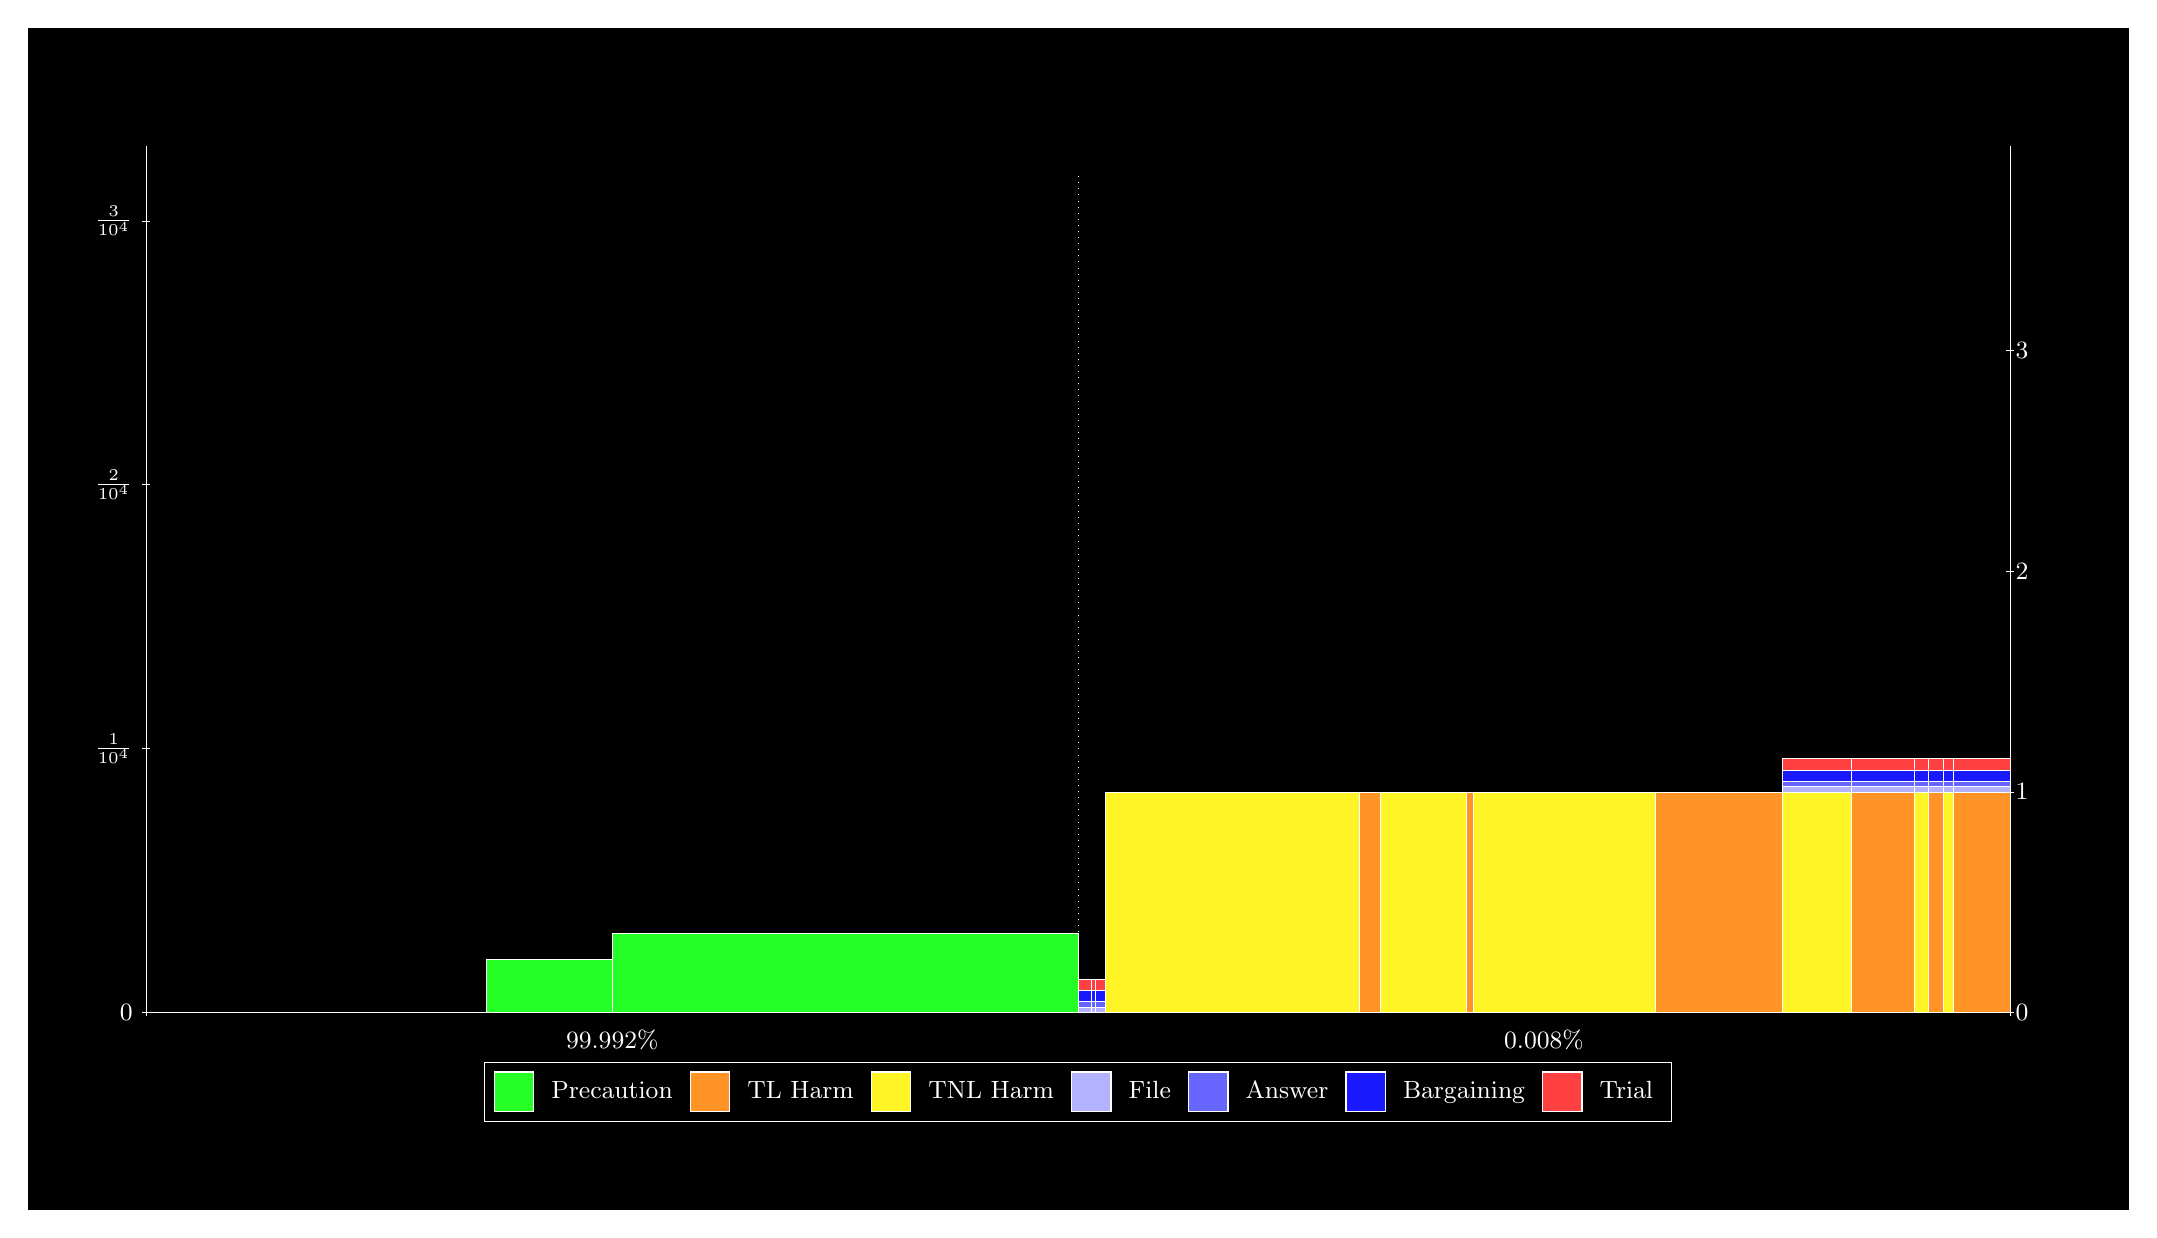
\begin{tikzpicture}
\draw[fill=black] (0,0) rectangle (26.667,15);
\draw[fill=green!85,draw=white,very thin] (5.8205,2.5) rectangle (7.4166,3.1703);
\draw[fill=green!85,draw=white,very thin] (7.4166,2.5) rectangle (13.333,3.5054);
\draw[fill=blue!30,draw=white,very thin] (13.333,2.5) rectangle (13.501,2.57);
\draw[fill=blue!60,draw=white,very thin] (13.333,2.57) rectangle (13.501,2.6401);
\draw[fill=blue!90,draw=white,very thin] (13.333,2.6401) rectangle (13.501,2.7802);
\draw[fill=red!75,draw=white,very thin] (13.333,2.7802) rectangle (13.501,2.9203);
\draw[fill=green!85,draw=white,very thin] (13.501,2.5) rectangle (13.549,2.5001);
\draw[fill=blue!30,draw=white,very thin] (13.501,2.5001) rectangle (13.549,2.5701);
\draw[fill=blue!60,draw=white,very thin] (13.501,2.5701) rectangle (13.549,2.6401);
\draw[fill=blue!90,draw=white,very thin] (13.501,2.6401) rectangle (13.549,2.7802);
\draw[fill=red!75,draw=white,very thin] (13.501,2.7802) rectangle (13.549,2.9203);
\draw[fill=green!85,draw=white,very thin] (13.549,2.5) rectangle (13.681,2.5001);
\draw[fill=blue!30,draw=white,very thin] (13.549,2.5001) rectangle (13.681,2.5701);
\draw[fill=blue!60,draw=white,very thin] (13.549,2.5701) rectangle (13.681,2.6402);
\draw[fill=blue!90,draw=white,very thin] (13.549,2.6402) rectangle (13.681,2.7803);
\draw[fill=red!75,draw=white,very thin] (13.549,2.7803) rectangle (13.681,2.9203);
\draw[fill=yellow!85,draw=white,very thin] (13.681,2.5) rectangle (16.906,5.3017);
\draw[fill=orange!85,draw=white,very thin] (16.906,2.5) rectangle (17.17,5.3017);
\draw[fill=green!85,draw=white,very thin] (17.17,2.5) rectangle (18.269,2.5001);
\draw[fill=yellow!85,draw=white,very thin] (17.17,2.5001) rectangle (18.269,5.3018);
\draw[fill=green!85,draw=white,very thin] (18.269,2.5) rectangle (18.354,2.5001);
\draw[fill=orange!85,draw=white,very thin] (18.269,2.5001) rectangle (18.354,5.3018);
\draw[fill=green!85,draw=white,very thin] (18.354,2.5) rectangle (20.665,2.5001);
\draw[fill=yellow!85,draw=white,very thin] (18.354,2.5001) rectangle (20.665,5.3018);
\draw[fill=green!85,draw=white,very thin] (20.665,2.5) rectangle (22.27,2.5001);
\draw[fill=orange!85,draw=white,very thin] (20.665,2.5001) rectangle (22.27,5.3018);
\draw[fill=yellow!85,draw=white,very thin] (22.27,2.5) rectangle (23.155,5.3017);
\draw[fill=blue!30,draw=white,very thin] (22.27,5.3017) rectangle (23.155,5.3717);
\draw[fill=blue!60,draw=white,very thin] (22.27,5.3717) rectangle (23.155,5.4418);
\draw[fill=blue!90,draw=white,very thin] (22.27,5.4418) rectangle (23.155,5.5819);
\draw[fill=red!75,draw=white,very thin] (22.27,5.5819) rectangle (23.155,5.722);
\draw[fill=orange!85,draw=white,very thin] (23.155,2.5) rectangle (23.949,5.3017);
\draw[fill=blue!30,draw=white,very thin] (23.155,5.3017) rectangle (23.949,5.3717);
\draw[fill=blue!60,draw=white,very thin] (23.155,5.3717) rectangle (23.949,5.4418);
\draw[fill=blue!90,draw=white,very thin] (23.155,5.4418) rectangle (23.949,5.5819);
\draw[fill=red!75,draw=white,very thin] (23.155,5.5819) rectangle (23.949,5.722);
\draw[fill=green!85,draw=white,very thin] (23.949,2.5) rectangle (24.132,2.5001);
\draw[fill=yellow!85,draw=white,very thin] (23.949,2.5001) rectangle (24.132,5.3018);
\draw[fill=blue!30,draw=white,very thin] (23.949,5.3018) rectangle (24.132,5.3718);
\draw[fill=blue!60,draw=white,very thin] (23.949,5.3718) rectangle (24.132,5.4418);
\draw[fill=blue!90,draw=white,very thin] (23.949,5.4418) rectangle (24.132,5.5819);
\draw[fill=red!75,draw=white,very thin] (23.949,5.5819) rectangle (24.132,5.722);
\draw[fill=green!85,draw=white,very thin] (24.132,2.5) rectangle (24.323,2.5001);
\draw[fill=orange!85,draw=white,very thin] (24.132,2.5001) rectangle (24.323,5.3018);
\draw[fill=blue!30,draw=white,very thin] (24.132,5.3018) rectangle (24.323,5.3718);
\draw[fill=blue!60,draw=white,very thin] (24.132,5.3718) rectangle (24.323,5.4418);
\draw[fill=blue!90,draw=white,very thin] (24.132,5.4418) rectangle (24.323,5.5819);
\draw[fill=red!75,draw=white,very thin] (24.132,5.5819) rectangle (24.323,5.722);
\draw[fill=green!85,draw=white,very thin] (24.323,2.5) rectangle (24.446,2.5001);
\draw[fill=yellow!85,draw=white,very thin] (24.323,2.5001) rectangle (24.446,5.3018);
\draw[fill=blue!30,draw=white,very thin] (24.323,5.3018) rectangle (24.446,5.3718);
\draw[fill=blue!60,draw=white,very thin] (24.323,5.3718) rectangle (24.446,5.4419);
\draw[fill=blue!90,draw=white,very thin] (24.323,5.4419) rectangle (24.446,5.582);
\draw[fill=red!75,draw=white,very thin] (24.323,5.582) rectangle (24.446,5.722);
\draw[fill=green!85,draw=white,very thin] (24.446,2.5) rectangle (25.167,2.5001);
\draw[fill=orange!85,draw=white,very thin] (24.446,2.5001) rectangle (25.167,5.3018);
\draw[fill=blue!30,draw=white,very thin] (24.446,5.3018) rectangle (25.167,5.3718);
\draw[fill=blue!60,draw=white,very thin] (24.446,5.3718) rectangle (25.167,5.4419);
\draw[fill=blue!90,draw=white,very thin] (24.446,5.4419) rectangle (25.167,5.582);
\draw[fill=red!75,draw=white,very thin] (24.446,5.582) rectangle (25.167,5.722);
\draw[white,very thin] (1.5,2.5) -- (1.5,13.5);
\draw[white,very thin] (1.45,2.5) -- (1.55,2.5);
\node[font=\small,text=white, anchor=east] at (1.45, 2.5) {0};
\draw[white,very thin] (1.45,5.8514) -- (1.55,5.8514);
\node[font=\small,text=white, anchor=east] at (1.45, 5.8514) {$\frac{1}{10^{4}}$};
\draw[white,very thin] (1.45,9.2029) -- (1.55,9.2029);
\node[font=\small,text=white, anchor=east] at (1.45, 9.2029) {$\frac{2}{10^{4}}$};
\draw[white,very thin] (1.45,12.554) -- (1.55,12.554);
\node[font=\small,text=white, anchor=east] at (1.45, 12.554) {$\frac{3}{10^{4}}$};

\draw[white,dotted,very thin] (13.333,2.83) -- (13.333,13.17);
\draw[white,very thin] (25.167,2.5) -- (25.167,13.5);
\draw[white,very thin] (25.117,2.5) -- (25.217,2.5);
\node[font=\small,text=white, anchor=west] at (25.117, 2.5) {0};
\draw[white,very thin] (25.117,5.3017) -- (25.217,5.3017);
\node[font=\small,text=white, anchor=west] at (25.117, 5.3017) {1};
\draw[white,very thin] (25.117,8.1034) -- (25.217,8.1034);
\node[font=\small,text=white, anchor=west] at (25.117, 8.1034) {2};
\draw[white,very thin] (25.117,10.905) -- (25.217,10.905);
\node[font=\small,text=white, anchor=west] at (25.117, 10.905) {3};

\draw[white,very thin] (1.5,2.5) -- (25.167,2.5);
\draw[white,very thin] (1.5,2.45) -- (1.5,2.55);
\node[font=\small,text=white, anchor=north] at (1.5, 2.45) {};
\draw[white,very thin] (25.167,2.45) -- (25.167,2.55);
\node[font=\small,text=white, anchor=north] at (25.167, 2.45) {};

\node[font=\small,text=white,anchor=south] at (7.4167, 1.9) {99.992\%};
\node[font=\small,text=white,anchor=south] at (19.25, 1.9) {0.008\%};
\draw (13.3333,2.5) node (B) {};
\begin{scope}[align=center]
\matrix[scale=0.5,draw=white,below=0.5cm of B,nodes={draw},column sep=0.1cm]{
\node[rectangle,draw,minimum width=0.5cm,minimum height=0.5cm,fill=green!85]{}; & \node[draw=none,font=\small,text=white]{Precaution}; &
\node[rectangle,draw,minimum width=0.5cm,minimum height=0.5cm,fill=orange!85]{}; & \node[draw=none,font=\small,text=white]{TL Harm}; &
\node[rectangle,draw,minimum width=0.5cm,minimum height=0.5cm,fill=yellow!85]{}; & \node[draw=none,font=\small,text=white]{TNL Harm}; &
\node[rectangle,draw,minimum width=0.5cm,minimum height=0.5cm,fill=blue!30]{}; & \node[draw=none,font=\small,text=white]{File}; &
\node[rectangle,draw,minimum width=0.5cm,minimum height=0.5cm,fill=blue!60]{}; & \node[draw=none,font=\small,text=white]{Answer}; &
\node[rectangle,draw,minimum width=0.5cm,minimum height=0.5cm,fill=blue!90]{}; & \node[draw=none,font=\small,text=white]{Bargaining}; &
\node[rectangle,draw,minimum width=0.5cm,minimum height=0.5cm,fill=red!75]{}; & \node[draw=none,font=\small,text=white]{Trial}; \\\\
};\end{scope}

\end{tikzpicture}
\end{document}